\section{Navigation Outcomes, Runtime Checks, and Trajectory Cases}
\label{app:navigation}

\begin{figure*}[!t]
\centering
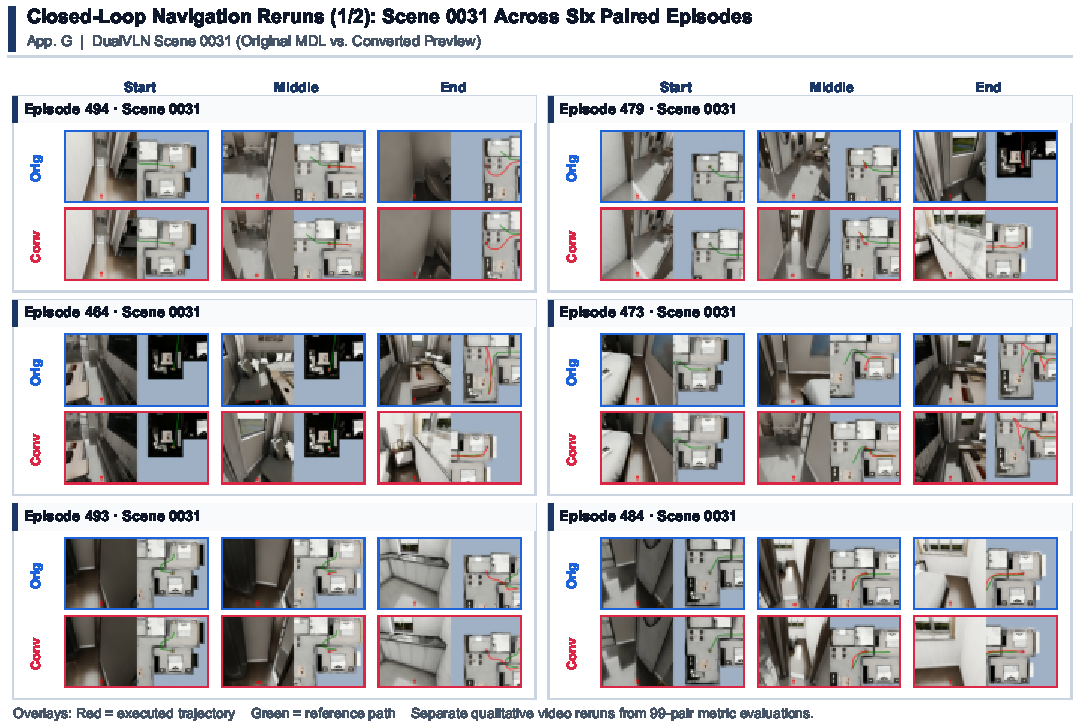
\includegraphics[width=0.86\textwidth]{app_fig6_nav_plate1.pdf}
\caption{\textbf{Consolidated closed-loop navigation reruns (1/2): \textsc{KuJiaLe Scene 0031}.}
Six paired episode recordings comparing \original{} (\textsc{MDL}) against \converted{} (\usdps{}) across \emph{Start}, \emph{Middle}, and \emph{End} frames with top-down occupancy maps (red: executed route; green: reference path). Recordings are separate qualitative reruns sharing episode IDs with the 99-pair metric benchmark.}
\label{fig:app-navcases1}
\end{figure*}

To examine how individual trajectory metrics co-vary under shader lowering, we inspect the full closed-loop evaluation across 99 paired episode IDs spanning \textsc{KuJiaLe} scenes \texttt{0031}, \texttt{0036}, and \texttt{0066} ($33$ episodes per scene), holding language instructions, start states, and policy weights fixed across \original{} and \converted{}. Table~\ref{tab:app-navfull} adds oracle success, step counts, fall/stuck fractions, and 95\% paired bootstrap confidence intervals to the main summary: aggregate \textsc{SR} ($-4.04$~pp), \textsc{SPL} ($-4.41$~pp), and oracle success ($-5.05$~pp) shift modestly while $30/99$ episodes reverse binary pass/fail outcomes ($17$ success-to-failure, $13$ failure-to-success) alongside an increase of $+41.75$ mean action steps. Separate fresh-launch simulator checks ($9$ loads per condition across all $3$ scenes; Table~\ref{tab:app-navload}) verify comparable initialization time ($13.95\,\mathrm{s}$ vs.\ $14.12\,\mathrm{s}$), warm-up frame rate ($2.36$ vs.\ $2.42\,\mathrm{FPS}$), and GPU footprint ($3{,}807$ vs.\ $3{,}829\,\mathrm{MB}$).

\begin{table*}[!t]
\centering\scriptsize
\begin{minipage}[t]{0.49\textwidth}
\centering
\setlength{\tabcolsep}{4pt}
\resizebox{\linewidth}{!}{% Generated by appendix/build_tables.py; source hashes in table_sources.json.
\begin{tabular}{lrrrr}
\toprule
Metric & Original & Converted & $\Delta$ & 95\% paired CI \\
\midrule
SR (\%) & 52.530 & 48.480 & -4.040 & [-15.150, 7.070] \\
SPL (\%) & 47.390 & 42.980 & -4.410 & [-14.170, 5.140] \\
Oracle success (\%) & 66.670 & 61.620 & -5.050 & [-15.150, 5.050] \\
Navigation error & 3.680 & 3.631 & -0.049 & [-0.646, 0.539] \\
Trajectory length & 6.975 & 7.060 & +0.084 & [-0.737, 0.930] \\
Action steps & 233.647 & 275.394 & +41.748 & --- \\
Fall rate & 0.020 & 0.020 & +0.000 & --- \\
Stuck rate & 0.000 & 0.000 & +0.000 & --- \\
\bottomrule
\end{tabular}
}
\caption{Full closed-loop navigation metrics across all 99 paired \textsc{DualVLN} episodes (differences reported as \converted{} minus \original{}, with 95\% paired bootstrap CIs where retained).}
\label{tab:app-navfull}
\end{minipage}\hfill
\begin{minipage}[t]{0.48\textwidth}
\centering
\setlength{\tabcolsep}{3pt}
\resizebox{\linewidth}{!}{% Generated by appendix/build_tables.py; source hashes in table_sources.json.
\begin{tabular}{lrrrr}
\toprule
Condition & Loads & Ready time (s) & Warm-up FPS & GPU memory (MB) \\
\midrule
Original & 9/9 & 13.95 [11.64, 16.28] & 2.36 [2.01, 2.70] & 3807 [3748, 3862] \\
Converted & 9/9 & 14.12 [12.31, 16.24] & 2.42 [2.08, 2.73] & 3829 [3689, 3971] \\
\bottomrule
\end{tabular}
}
\caption{Fresh-launch simulator initialization, frame rate, and GPU memory checks ($9$ runs per condition across scenes \texttt{0031}, \texttt{0036}, and \texttt{0066}).}
\label{tab:app-navload}
\end{minipage}
\end{table*}

\begin{figure*}[!t]
\centering
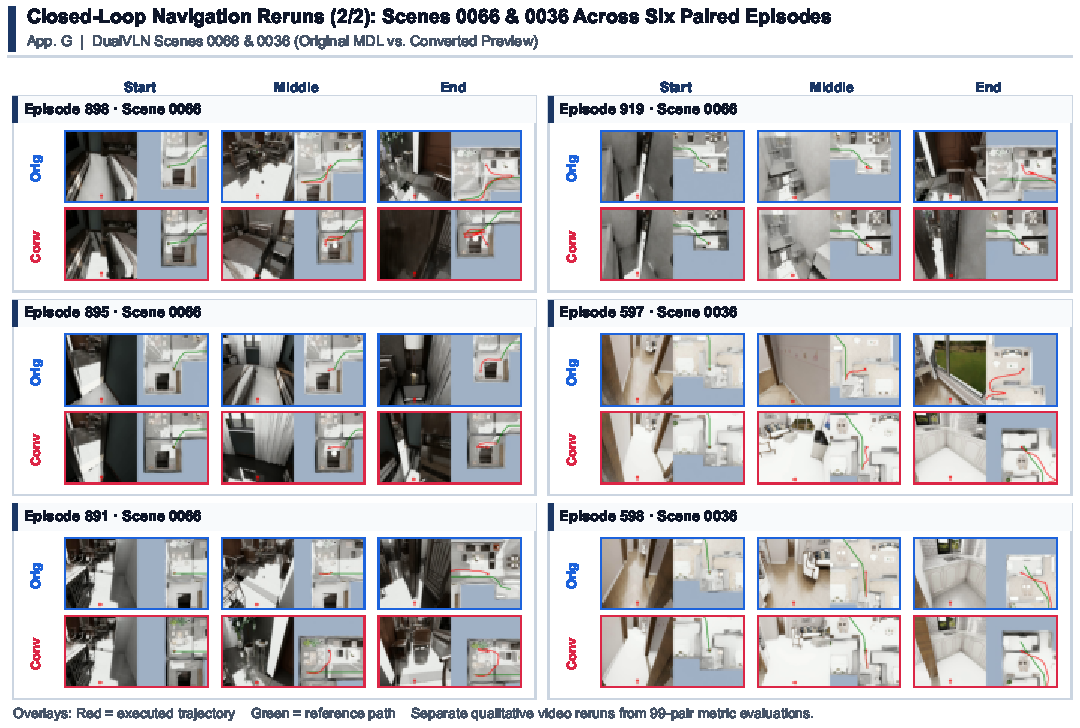
\includegraphics[width=0.84\textwidth]{app_fig7_nav_plate2.pdf}
\caption{\textbf{Consolidated closed-loop navigation reruns (2/2): \textsc{KuJiaLe Scenes 0066 \& 0036}.}
Six paired episode recordings from scenes \texttt{0066} and \texttt{0036} matching the layout of Figure~\ref{fig:app-navcases1}. Minor shader-induced observation shifts can trigger divergent room-entry timing and early termination even on shared start states and instructions.}
\label{fig:app-navcases2}
\end{figure*}

\subsection{Twelve paired recorded trajectory examples}
Figures~\ref{fig:app-navcases1} and~\ref{fig:app-navcases2} consolidate all 12 qualitative video reruns into two panoramic plates across all three scenes, covering asymmetric failures, divergent trajectories sharing identical final binary status, and consistent routes. For example, in episode~898 (scene~\texttt{0066}), the converted rollout loops near the entryway while the original rollout reaches deeper rooms; in episode~891, the converted agent takes a wide kitchen detour; whereas episode~598 terminates near matched kitchen viewpoints under both shaders. Because each metric rollout executed a single closed-loop trajectory per shader condition, these episode outcomes reflect both shader shifts and single-rollout controller dynamics.
